\documentclass{article}
\usepackage[utf8]{inputenc}
\usepackage[italian]{babel}
\usepackage{amsmath}
\usepackage{amsfonts}
\usepackage{amssymb}
\usepackage{natbib}
\usepackage{graphicx}
\usepackage{caption}
\captionsetup[figure]{labelformat=empty}


\title{Integrazione numerica}
\author{Arment Pelivani, Lorenzo D'Agostino}
\date{2019}


\begin{document}
\maketitle
\begin{center}
\begin{figure}[ht]


\includegraphics[scale=0.6]{img/math-emporium.jpg} 
\label{fig:trasl}
\end{figure}

\end{center}

\newpage
\tableofcontents
\newpage
\section{Introduzione}
In analisi numerica le formule di integrazione, o formule di quadratura, consistono in una serie di metodi che stimano il valore di un integrale definito senza la necessità di dover calcolare la primitiva della funzione integranda.

Parliamo di approssimazione in quanto gli algoritmi ed i risultati da essi generati, in generale, sono sottoposti ad errori di vario tipo:

\begin{itemize}
\item Errori di approssimazione: 

- si verificano quando arrotondiamo numeri per eccesso o per difetto.
\item Errori umani: 

- non prevedibili, in quanto si verificano nel momento in cui l'utente inserisce i dati di imput.
\item Errori di troncamento: 

- si verificano nel momento in cui tronchiamo i numeri, ad una certa cifra decimale, senza arrotondare.
\item Errori di overflow: 

- si verificano nel momento in cui si supera il limite di dimensione massima dello stack. Tipico delle funzioni ricorsive, è evitabile effettuando controlli accurati.
\end{itemize}

Negli algoritmi proposti verranno considerate soluzioni alle problematiche sopra descritte, ed anche una valutazione sulla complessità computazionale degli stessi.
A tal proposito utilizzeremo la notazione \textit{\textbf{O-grande}} per valutare la complessità computazionale degli algoritmi proposti valutandola nel caso peggiore.

\begin{center}
\begin{figure}[ht]

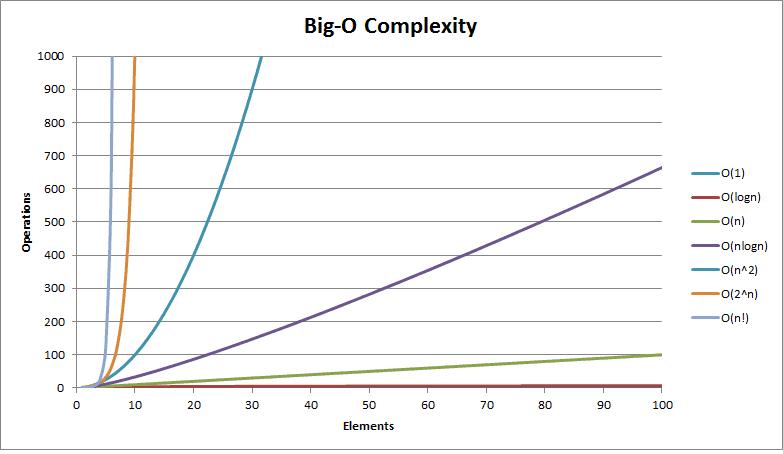
\includegraphics[scale=0.39]{img/big-o-complexity.png} 
\label{fig:complex}
\end{figure}

\end{center}
\newpage
La necessità di utilizzare le formule di quadratura deriva da diversi motivi:
\begin{itemize}
\item non tutte le funzioni ammettono primitiva in forma esplicita.
\item la primitiva può essere molto complicata da valutare.
\item la funzione è disponibile solo per punti.
\end{itemize}
Distinguiamo le formule di quadratura in due grandi categorie: le formule di Newton-Cotes, e le formule di Gauss.

nel seguente articolo ci soffermeremo sulle prime citate sopra con un accenno anche al metodo di Montecarlo utilizzato soprattutto per funzioni di piu variabili.

In generale i metodi numerici non stocastici trovano una soluzione al problema seguendo la definizione dell'integrale di Riemann, suddividendo quindi l'intervallo di integrazione in una molteplicità di sottointervalli valutando poi la funzione stessa in più punti.

Tutti i metodi studiati verranno implementati attraveso l'utilizzo del linguaggio java.

\begin{center}
\begin{figure}[ht]

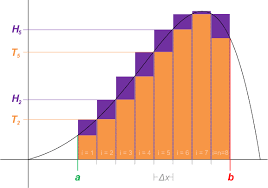
\includegraphics[scale=1]{img/rieman.png} 
\label{fig:rieman}
\end{figure}

\end{center}

\newpage
\section{Il metodo dei rettangoli}
Il primo metodo che studiamo è il più semplice, ma anche il meno preciso. L’intervallo di integrazione viene suddiviso in un numero finito di parti, che quindi sono piccole ma non infinitesime.
\begin{figure}[ht]
\centering
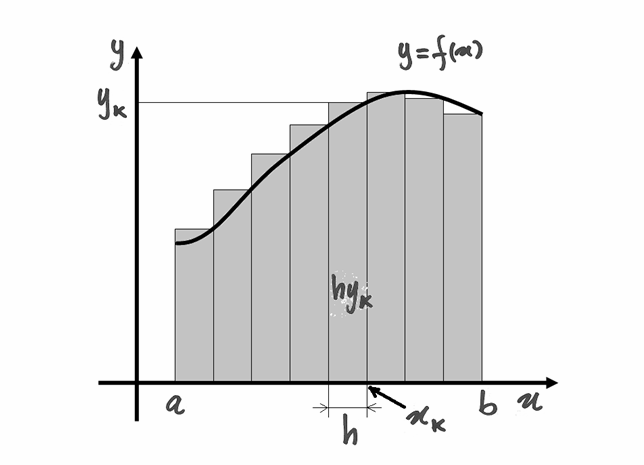
\includegraphics[scale=0.25]{img/09_01_int_rettangoli.png} 
\label{fig:rect}
\end{figure}

Data la funzione continua $f:[a,b]\rightarrow \mathbb{R}$ costruiamo una successione di $n$ punti tali che $a=x_0<x_1<x_2<...<x_n=b$.
In ogni sottointervallo $[x_k,x_{k+1}]$ prendiamo un numero $\bar{x_k}$ e approssimiamo l'integrale $\int_{a}^{b}f(x)dx$ con la somma $\sum_{0}^{n-1}f(\bar{x_k}*h$ dove $h = \frac{b-a}{n}$ supposti tutti i sottointervalli uguali.

Se prendiamo come altezza di ogni rettangolo il valore della funzione nell'estremo destro della base, $\bar{x_k} = x_{k+1} , f(x_k)=y_k$. $h*y_k$ è l’area di ogni rettangolo e la somma che approssima l’integrale diventa: \[\sum_{0}^{n-1}f(x_{k+1})*h = h*\sum_{0}^{n-1}y_{k+1}=h*\sum_{1}^{n}y_k\].

Risulta perciò l'uguagliaza approssimata: \[\int_a^bf(x)dx\cong h*\sum_1^ny_k\]

Dalle precedenti considerazioni ne segue il codice:
codice c++

\subsection{Esempio}
$\int_0^3x^2dx$
Calcoliamo con questo metodo un integrale facile: $S=\int_0^3x^2dx$, il cui valore esatto è 9.
\begin{align*}
&n=10,\quad S=10,395\\
&n=100,\quad S=9,13545\\
&n=1000,\quad S=9,0135045\\
&n=10000,\quad S=9,00135005
\end{align*}

Man mano che cresce il numero degli intervalli, e l’algoritmo prevede un maggior numero di cicli, il risultato approssima sempre meglio quello esatto.

\newpage
\section{Il metodo dei trapezi}
Come indica il nome, questo metodo si basa sulla sostituzione dei rettangoli con i trapezi. Il grafico della funzione viene approssimato da una spezzata, che è il grafico di una funzione approssimante $\phi$, una funzione lineare a tratti. In pratica il valore di $\int_a^bf(x)dx$ si approssima con il valore esatto di $\int_a^b\phi(x)dx$.

$\int_a^bf(x)dx\cong\int_a^b\phi(x)dx$.

Manteniamo la stessa suddivisione in intervalli adottata con il metodo dei rettangoli. Data $y_k~=~f(x_k)$, definiamo la funzione $\phi$ come la funzione che ha per grafico la spezzata che unisce i punti $P_k(x_k,y_k),\ k=0 ... n$.

\begin{figure}[ht]
\centering
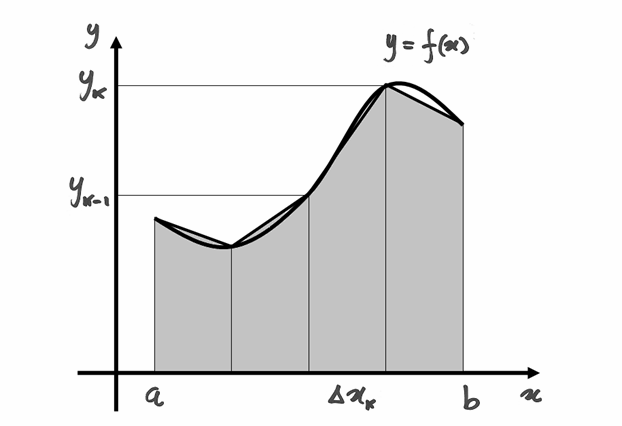
\includegraphics[scale=0.25]{img/09_02_int_trapezi.png} 
\label{fig:trap}
\end{figure}

L’area di ogni trapezio è data da $\frac{y_{k-1}+y_k}{2}\Delta x_k$, quindi

\begin{align*}
\frac{y_{k-1}+y_k}{2}\Delta x_k=&\int_{x_{k-1}}^{x_k}\phi(x)dx.\\
\int_a^bf(x)dx \cong \int_a^b\phi(x)dx=&\sum_1^n\int_{x_{k-1}}^{x_k}\phi(x)dx
\end{align*}

Possiamo quindi scrivere la formula approssimata
\[
\int_a^bf(x)dx\cong \frac{1}{2}\sum_1^n (y_{k-1}+y_k)\Delta x_k\]

Nella suddivisione in progressione aritmetica, ogni sottointervallo ha ampiezza costante: $\Delta x_k=h$ e quindi si ha:

\begin{align*}
\int_a^bf(x)dx\cong &\frac{h}{2}\sum_1^n (y_{k-1}+y_k)=\\
=&\frac{h}{2}[(y_0+y_1)+(y_1+y_2)+(y_2+y_3)+ ... +(y_{n-1}+y_n)]=\\
=&\frac{h}{2}(y_0+2y_1+2y_2+2y_3+ ... +2y_{n-1}+y_n)=\\
=&\frac{h}{2}\left[y_0+2\sum_1^{n-1}y_k+y_n \right]
\end{align*}

Ne segue il codice: 
codice

\subsection{Esempio}

Se si testa il funzionamento dell’algoritmo sulla funzione $y=x^2$ si scopre che per $n=10$, cioè ricoprendo la superficie con 10 trapezi, si ottiene quasi la stessa precisione ottenuta con 1000 rettangoli.

\begin{align*}
&n=10,\quad S=9,045\\
&n=100,\quad S=9,00045\\
&n=1000,\quad S=9,0000045\\
\end{align*}

\subsection{Complessità computazionale}
Per calcolare la complessità computazionale del metodo tralasceremo le operazioni di assegnazione, gli eventuali controlli del caso e i calcoli iniziali che risultano avere complessità pari a $O(1)$ che quindi non influenzano il risultato finale.

L'algoritmo proposto presenta al suo interno un unico ciclo \textit{for}, il cui numero di iterazioni $n$ dipende dal numero di sottointervalli che desideriamo generare per ottenere un' approssimazione più o meno precisa del valore dell' integrale stesso.

La complessità computazionale dell' algoritmo risulta per cui essere : \[T_{tot,worst} = O(n)\]

\newpage
\section{La formula di Simpson}
Con il ricoprimento a trapezi la funzione è stata trasformata in una funzione a dominio discreto e per ogni coppia di suoi punti al posto della funzione originale abbiamo usato una funzione lineare. Si è trattato quindi di una interpolazione lineare.

Procediamo ora, isolando non coppie ma terne di punti consecutivi e considerando, al posto della funzione, l’arco di parabola per quei punti. Il grafico che passa per tre punti è infatti espressione di un polinomio al massimo di secondo grado. Se dobbiamo considerare gruppi di tre punti, gli intervallini saranno necessariamente in numero pari, quindi $n=2m$. Limitiamoci anche questa volta a intervallini di uguale ampiezza h=$\frac{b-a}{2m}$.

Procediamo con i primi tre punti $x_0,x_1,x_2$ e poi cercheremo di generalizzare il risultato. Il fatto importante, però, non è tanto esprimere il polinomio, quanto il suo integrale in $[x_0,x_2]$. Stiamo infatti cercando di sostituire la funzione f con una funzione $\psi$ che coincide con l’unico polinomio passante per i tre punti consecutivi, che isolano una coppia di intervallini. E deve valere che l’integrale approssimato di $f$ è l’integrale esatto di $\psi$, il quale a sua volta è la somma di una coppia di integrali:
\[
\int_a^b\psi(x)dx=\sum_1^m\int_{x_{2k-2}}^{x_{2k}}\psi(x)dx\]

Il primo di questi integrali è
\[
\int_{x_0}^{x_2}\psi(x)dx\]

La funzione $\psi(x)$, come abbiamo detto è un polinomio al massimo di secondo grado: $P(x)~=~Ax^2+Bx+C$, del quale sappiamo che $P(x_0)=y_0,\ P(x_1)=y_1,\ P(x_2)=y_2$, con A,B,C da ricavare.

Per facilitare la ricerca di questi tre coefficienti, ricordando che gli intervallini hanno uguale ampiezza $h$: potremo allora traslare i due intervallini: $x_0=-h,\ x_1=0,\ x_2=h$, mantenendo, ovviamente, uguali valori di $y$ corrispondenti.

\begin{figure}[ht]
\centering
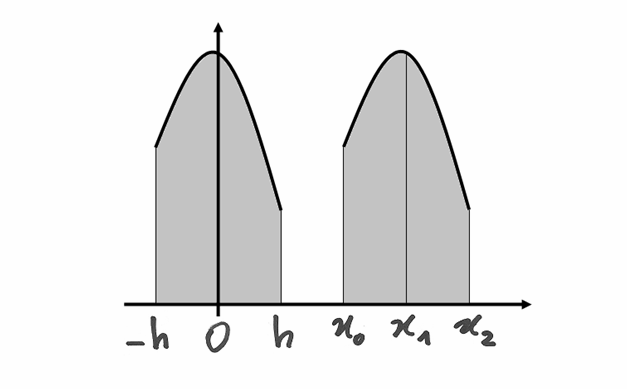
\includegraphics[scale=0.25]{img/09_04_simmetria.png} 
\label{fig:trasl}
\end{figure}

Il vantaggio di questa trasformazione è che ora dobbiamo calcolare
\[
\int_{x_0}^{x_2}\psi(x)dx=\int_{-h}^{h}P(x)dx=\int_{-h}^{h}(Ax^2+Bx+C)dx=
\int_{-h}^{h}Ax^2dx+\int_{-h}^{h}Bxdx+\int_{-h}^{h}Cdx\]

Poiché ora abbiamo l’intervallo di integrazione simmetrico, le funzioni dispari hanno integrale nullo mentre le funzioni pari hanno integrale doppio rispetto all’integrale su metà intervallo:
\[
\int_{-h}^{h}(Ax^2+Bx+C)dx= 2 \int_0^{h}(Ax^2+C)dx
=2\left[\frac{Ah^3}{3}+Cx\right]_0^h=\frac{2}{3}Ah^3+2Ch.\]

Abbiamo così scoperto che il calcolo di B non è importante. Poi, da $P(0)=C$ segue $C=y_1$. Per il calcolo di $A$:

\begin{align*}
&P(-h)=Ah^2-Bh+C=y_0\\
&P(h)=Ah^2+Bh+C=y_2\\
&P(-h)+P(h)=2Ah^2+2C=y_0+y_2\\
&2Ah^2=y_0-2y_1+y_2\\
&\int_{-h}^{h}(Ax^2+Bx+C)dx=\frac{2}{3}Ah^3+2Ch=\frac{h}{3}\left[2Ah^2+6C \right]=
\frac{h}{3}(y_0+4y_1+y_2)
\end{align*}

Abbiamo quindi trovato l’integrale dell’arco di parabola per i primi tre punti, in funzione dell’ampiezza $h$ degli intervallini e delle ordinate dei tre punti. La cosa si estende facilmente a tutte le terne di punti successive, così:

\begin{align*}
\int_a^bf(x)dx\cong &\frac{h}{3}(y_0+4y_1+y_2)+\frac{h}{3}(y_2+4y_3+y_4)+ ...=\\
=&\frac{h}{3}(y_0+4y_1+2y_2+4y_3+2y_4+ ... +2y_{n-2}+4y_{n-1}+y_n)
\end{align*}

Tranne che per il primo e per l’ultimo termine, sui termini di indice pari si raddoppia la somma, mentre sui termini di indice dispari si quadruplica. Ricordando che $n=2m$, riscriviamo e sintetizziamo:

\begin{align*}
\int_a^bf(x)dx\cong &\frac{h}{3}(y_0+4y_1+2y_2+ ... +2y_{2m-2}+4y_{2m-1}+y_{2m})=\\
&=\frac{h}{3}\left[y_0+4\sum_1^m y_{2k-1}+2\sum_1^{m-1}y_{2k}+y_{2m} \right]
\end{align*}

Da cui ne deriva il codice: 
codice

\subsection{Confronto tra i metodi}

Vale la pena di testare i tre metodi descritti, per calcolare un integrale di cui non conosciamo la primitiva: $\int_0^2e^{-x^2}dx$.

\hfill

\begin{tabular}{ |p{3cm}||p{3cm}|p{3cm}|p{3cm}|  }
 \hline
 \multicolumn{4}{|c|}{Confronto Algoritmi} \\
 \hline
 \textbf{Intervalli}& \textbf{Rettangoli} & \textbf{Trapezi}& \textbf{Simpson}\\
 \hline
10  & 0,71460477    &0,7462108&  0,74682495\\
 20&   ...  & ...  &0,74682418\\
 40 &... & ...&  0,74682414\\
 1000    &0,74650801 & 0,74682407&  ...\\
 10000&   ...  & 0,74682413 & ...
\\
 1000000& 0,74682382  & ...   &...\\
 \hline
\end{tabular}

\hfill

Dai risultati descritti nella tabella possiamo notare come il metodo Di Simpson risulta convergere al risultato esatto molto più rapidamente degli altri due metodi che necessitano di un numero di intervalli molto superiore per avvicinarsi al risultato ottenuto dall'algoritmo di Simpson con 40 intervalli.

\subsection{Complessità computazionale}

Per calcolare la complessità computazionale del metodo tralasceremo le operazioni di assegnazione, gli eventuali controlli del caso e i calcoli iniziali che risultano avere complessità pari a $O(1)$ che quindi non influenzano il risultato finale.

Il primo ciclo che incontriamo all' interno del codice risulta avere complessità computazionale pari a \[T_{for_1,worst} = O(n)\]

Proseguendo nell'algoritmo incontriamo un \textit{do-while} la cui complessità computazionale $T_{do-while,worst}$ dipenderà dal numero massimo $n_{max}$ di iterazioni che l' utente permetterà di eseguire al programma e dalla precisione richiesta sempre dall' utente (che però non influenza il calcolo). All'interno del ciclo \textit{do-while} incontriamo anche un secondo ciclo \textit{for} la cui complessità sarà poi inclusa nel calcolo della precedente: \[T_{for_2,worst} = O(n)\]. La complessità finale del ciclo \textit{do-while} risulta quindi essere : \[T_{do-while,worst} = O(n_{max}*T_{for_2,worst} = O(n_{max}*O(n))\]
Di conseguenza, la complessità totale dell'algoritmo nel caso peggiore risulta essere : \[T_{tot,worst} = T_{for_1,worst})+T_{do-while,worst} = O(n)+O(n_{max}*O(n)) =O(n_{max}*O(n))\]

\newpage

\section{Il metodo Montecarlo}
Gli algoritmi di quadratura studiati fino ad ora si basano comunque su una impostazione geometrica alla risoluzione del problema di partenza. L'algoritmo che andremo a studiare ora (Montecarlo) ha un’impostazione del tutto differente dai precedenti. Proviene infatti da studi di tipo stocastico/probabilistico e il suo nome ricorda il gioco d’azzardo ed i numeri casuali.

Consideriamo una funzione $f$ continua e positiva su $[a,b$] e conosciamo anche un maggiorante della funzione, cioè un numero $M$ tale che$ f(x)\le M$ $\forall x\in [a,b]$. Il trapezoide della funzione è certamente contenuto nel rettangolo di base avente l’intervallo $[a,b]$ e altezza $M$.

Ciò che ci proponiamo di fare è geneare $n$ numeri casuali, all'interno del rettangolo descritto sopra, e stimare opportunamente l'area sottesa alla curva considerata a partire dalla percentuale $\frac{m}{n}$ di numeri casualmente generati contenuti all'interno dell'area da stimare.

\begin{figure}[ht]
\centering
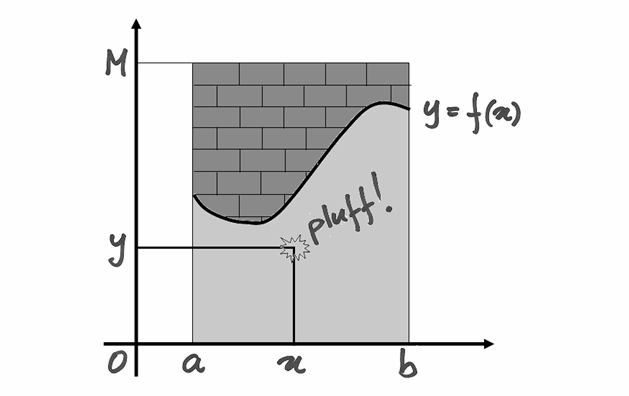
\includegraphics[scale=0.25]{img/09_06_pluff.png} 
\label{fig:Montecarlo}
\end{figure}\

A questo punto, la stima del risultato risulta essere: 
\[
\int_a^bf(x)dx=\frac{m}{n}(b-a)M.
\]
I valori generati devono essere quindi casuali e distribuiti in modo omogeneo su tutto il rettangolo, quindi le loro coordinate devono essere calcolate da una funzione opportuna, che fornisce numeri uniformemente distribuiti (in ogni porzione dell’intervallo cade più o meno la stessa quantità di numeri) e indipendenti (ogni numero non è legato al numero generato in precedenza). Se queste caratteristiche sono rispettate, allora il caso viene simulato abbastanza bene. Nel linguaggio c++ esiste un algoritmo apposito che garantisce un buon rispetto di queste regole. La funzione in c++ che implementa la generazione di questi numeri è detta random e verrà indicata con il termine $\mathit{rnd}$.

Dunque, dobbiamo generare casualmente punti nel rettangolo $[a,b]\times[0,m]$, con il generatore di numeri pseudocasuali rnd, che fornisce numeri fra 0 e 1. Avremo quindi coppie di numeri da trasformare, in modo che risultino appartenere all’intervallo voluto. La funzione che trasforma questi numeri è una semplice retta. Infatti, perché un numero casuale $\mathit{rnd} \in [0,1]$ sia trasformato in un numero dell’intervallo  $x\in[a,b]$, deve valere che
\[
X=(b-a)\mathit{rnd}+a.\]

\begin{figure}[ht]
\centering
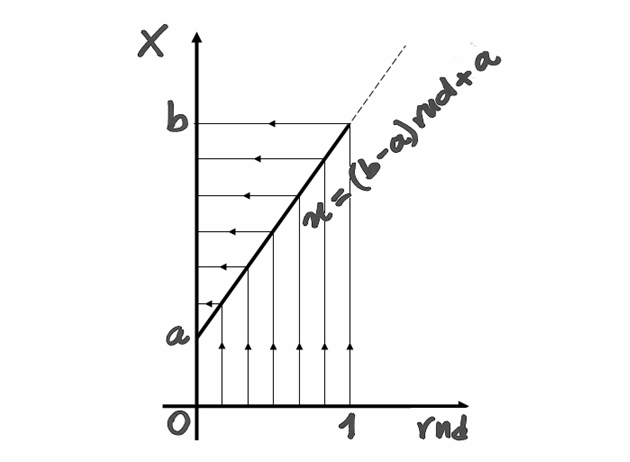
\includegraphics[scale=0.25]{img/09_07_f_rnd.png} 
\label{fig:RandomTransform}
\end{figure}\

Per costruire l’algoritmo che conta quanti punti casuali appartengono all’area richiesta abbiamo bisogno di controllare se la coordinata $Y$ dei punti è nel trapezoide, cioè se ha valore inferiore a quello corrispondente della funzione: $Y<f(x)$.

L’algoritmo riceve in ingresso il numero $n$ di lanci, cioè di valori casuali da generare, e gli intervalli entro cui trasformarli. Poi incrementa un contatore $m$ ogni volta che il numero $y$ è inferiore a $f(x$) e infine produce la frazione $\frac{m}{n}$ che, moltiplicata per l’area del rettangolo, fornisce la stima dell’integrale.

codice

\subsection{Esempio di metodo Montecarlo}

Proviamo il metodo sul calcolo di $\int_0^3 x^2dx$ e confrontiamolo con i risultati dei metodi precedenti e con il risultato esatto che conosciamo, cioè 9. Come maggiorante useremo $M=9$.

\hfill

\begin{tabular}{ |p{3cm}||p{3cm}|}
 \hline
 \multicolumn{2}{|c|}{Montecarlo} \\
 \hline
 \textbf{Numeri casuali}& \textbf{Algoritmo}\\
 \hline
10  & 8,1   \\
 100&   10,8 \\
 1000 &8,937\\
 10000    & 9,0315 \\
 100000&   8,99532 \\
 1000000& 8,967537 \\
 \hline
\end{tabular}

\hfill

Osserviamo che il metodo è impreciso e non è detto che all'aumentare dei numeri generati migliori la precisione. Si tratta di un metodo statistico, cioè che produce risultati in media vicini al valore esatto. Infatti lo numero di valori generati non dà, in genere, lo stesso risultato. Bisogna quindi ripetere gli esperimenti e fare la media.

\subsection{Complessità computazionale}

Per calcolare la complessità computazionale del metodo tralasceremo le operazioni di assegnazione, gli eventuali controlli del caso e i calcoli iniziali che risultano avere complessità pari a $O(1)$ che quindi non influenzano il risultato finale.

\end{document}